\lab{Uniform Motion}

\section*{Displacement}

The displacement of an object is its change in position. It is defined as:

\begin{eqnarray*}
	\mbox{displacement} & = & \mbox{final position coordinates} - \mbox{initial position coordinates} \\
	\Delta \vect{r} & = & \vectsub{r}{f} - \vectsub{r}{i} \\
\end{eqnarray*}

\noindent
(Remember that the coordinates themselves are a vector so we are really subtracting vector quantities in this equation.)  Suppose that in an animation, a car moves to the right as shown in Figure \ref{uniform-motion/vw-disp}. Its final position coordinates are (+2,+3) m. Its initial position coordinates are (-4,+3) m. Thus, the displacement of the car is:  $\mbox{displacement} = (2,3)\ \meter - (-4,3)\ \meter = (+6,0) \ \m$

%\begin{eqnarray*}
%	\mbox{displacement} & = &(2,3)\ \meter - (-4,3)\ \meter = (+6,0) \ \m
%\end{eqnarray*}

\scaledimage{uniform-motion/vw-disp}{A car moves to the right.}{0.35}

An object's displacement is a vector whose tail is at the object's initial position and head is at the object's final position. The displacement of the car is the vector shown in Figure \ref{uniform-motion/vw-disp-vector}.

\scaledimage{uniform-motion/vw-disp-vector}{The car's displacement vector.}{0.35}

Since the displacement is  $(+6,0) \ \m$ and has zero y-component, then it must be a vector that is parallel to the x-axis and points 6 m to the right. Thus, the mathematical result agrees with the picture in Figure \ref{uniform-motion/vw-disp-vector}.

\subsection*{Example}

\tightframe{

{\bf Question:}

The top view of a pickup moving from $\vectsub{r}{1}$ to $\vectsub{r}{2}$ is shown below. Sketch and calculate the truck's displacement.\\

%\scaledimage{uniform-motion/pickup-disp-vector}{A pickup truck moves from $\vect{r}{1}$ to $\vect{r}{2}$.}{0.4}

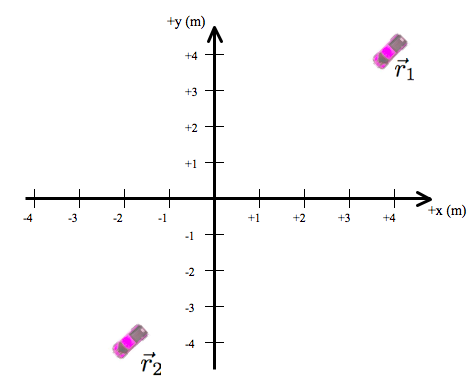
\includegraphics[scale=0.5]{uniform-motion/pickup-disp}


{\bf Answer:}

The displacement of the pickup is:

\begin{eqnarray*}
	\mbox{displacement} & = & \vectsub{r}{2} - \vectsub{r}{1}\\
	 & = &   (-2,-4)\ \meter - (+4,+4)\ \meter \\
	 & = & (-6, -8)\ \meter
\end{eqnarray*}

To sketch the displacement vector, draw an arrow from the initial position of the pickup to the final position of the pickup, as shown below.

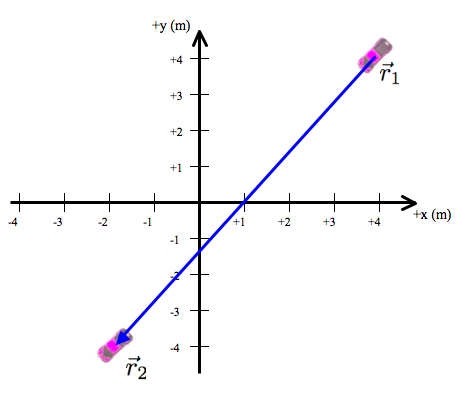
\includegraphics[scale=0.5]{uniform-motion/pickup-disp-vector}
}

\section*{Updating the position of an object}

When creating games or animation, you move objects on the screen. To move an object to some ``final'' coordinates, you take its initial coordinates and add a displacement.

\begin{eqnarray*}
	\mbox{final position coordinates} & = &  \mbox{initial position coordinates} + \mbox{displacement}
\end{eqnarray*}

Suppose that a toy pickup is at (+4,-2) m and you displace it (-3,0) m. Then, its new position is

\begin{eqnarray*}
	\mbox{final position coordinates} & = & (+4,-2) \ \meter + (-3,0)\ \meter \\
	& = & (+1,-2)\ \meter
\end{eqnarray*}

The position of the pickup at $\vectsub{r}{2}$ is shown in Figure \ref{uniform-motion/pickup-three}.

\scaledimage{uniform-motion/pickup-three}{A pickup is displaced (-3,0) m to the left.}{0.5}

\subsection*{Example}

\tightframe{

{\bf Question:}

Suppose that a toy pickup is at (+4,-2) m and you displace it (-3,0) m. Let's call this \emph{step 1}.  After two \emph{additional} steps, what will be the position of the pickup? \\

{\bf Answer:}

There is a total of three ``steps''. After the first step, the pickup is at $(+4,-2) \ \meter + (-3,0)\ \meter=(+1,-2)\ \meter$. After the second step, the pickup is at $(+1,-2) \ \meter + (-3,0)\ \meter=(-2,-2)\ \meter$, as shown in Figure \ref{uniform-motion/pickup-three}. After the third step, the pickup is at $(-2,-2) \ \meter + (-3,0)\ \meter=(-5,-2)\ \meter$. 

It is a good idea to extend the axis in Figure \ref{uniform-motion/pickup-three} and sketch the location of the pickup at $\vectsub{r}{4}$.

}

\section*{Uniform motion}

Each step of the pickup shown in Figure \ref{uniform-motion/pickup-three} takes place in a time interval $\Delta t$. If you have a running clock to measure time, then the \emph{clock reading} when the pickup is at $\vectsub{r}{1}$ is $\ssub{t}{1}$. The clock reading when the pickup is at $\vectsub{r}{2}$ is $\ssub{t}{2}$. The \emph{time interval} $\Delta t$ (or time elapsed) is defined as the difference in the clock readings:

\begin{eqnarray*}
	\Delta t & = &t_2-t_1
\end{eqnarray*}

Suppose that we use the same time interval between successive displacements. If the object's displacement in equal time intervals is the same, then the result is called \emph{uniform motion}.  It's fairly easy to identify uniform motion because successive pictures of the object in equal time intervals are equally spaced apart, as shown in Figure \ref{uniform-motion/pickup-three} for the pickup.

For example, consider a simulation of a cart moving to the right on a track shown in Figure \ref{uniform-motion/constv-cart-2}. The dots represent the location of the center of the cart at a certain clock reading. Since the clock readings were made at equal time steps and since successive positions of the cart are equally spaced, the cart's motion is described as uniform motion.

\scaledimage{uniform-motion/constv-cart-2}{A cart on a track moves to the right with uniform motion.}{0.75}

Let's record the x-positions of the cart and the clock readings in a data table.

\begin{table}[htdp]
\caption{x-positions of the cart in Figure \ref{uniform-motion/constv-cart-2}.}
\begin{center}
\begin{tabular}{|c|c|}
\hline
t (s) & x (cm)  \\
\hline
\hline
0 & 15 \\
\hline
0.1 & 25 \\
\hline
0.2 & 35  \\
\hline
0.3 & 45  \\
\hline
0.4 & 55  \\
\hline
0.5 & 65  \\
\hline
\hline
\end{tabular}
\end{center}
\label{default}
\end{table}%

A graph of x as a function of time is shown in Figure \ref{uniform-motion/constv-graph}. You will notice that a best-fit ``curve'' through the data is a straight line. The ``rise'' is 10 cm for each ``run'' of 0.1 s. This gives a constant slope for the curve. The slope is

\begin{eqnarray*}
	slope & = & \frac{rise}{run} \\
	& = & \frac{10 \ \centi\meter}{0.1\ \second} \\
	& = & 100\ \centi\meter \per \second
\end{eqnarray*}

The slope means that the x-position of the cart increases 10 cm for each 0.1 s of time elapsed, or in other words, 100 cm in each 1 second elapsed. This is called the \emph{x-velocity} of the cart. 

Note that the graph of $x$ vs. $t$ doesn't tell us anything about the y-motion of the cart. In this case, the cart is moving horizontally, so its \emph{y-velocity} is zero. As a result, we can write the velocity of the cart as  $\vect{v}=(100,0)$ cm/s. But if we didn't know its y-velocity and all we had was the data for graph for $x(t)$, then we wouldn't know anything about the y-motion of the cart.

\scaledimage{uniform-motion/constv-graph}{A graph of x-position as a function of time for the cart.}{0.4}

\pagebreak

\subsection*{Example}

\tightframe{

{\bf Question:}

A graph for the x-position as a function of time for a cart on a track is shown below. \\

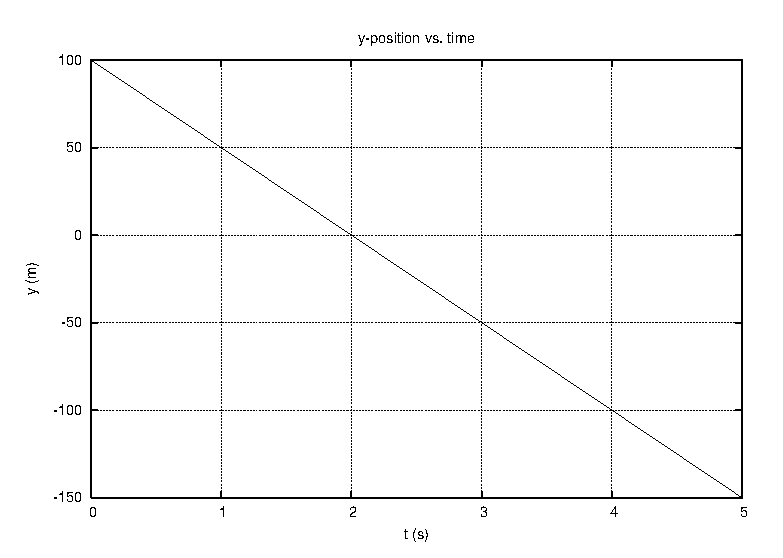
\includegraphics[scale=0.75]{uniform-motion/x-t-graph}

(a) What is the x-velocity of the cart? \\

(b) In which direction is the cart traveling? \\

(c) What can you say about the y-motion of the cart? \\

{\bf Answer:}

(a)  The x-velocity is the slope of the graph. Choose two points on the line. For example, you might choose (1 s, 20 cm) and (4 s, 5 cm).  The slop is

\begin{eqnarray*}
	slope & = & \frac{rise}{run} \\
	& = & \frac{(5-20) \ \centi\meter}{(4-1)\ \second} \\
	& = & \frac{-15 \ \centi\meter}{3\ \second} \\
	& = & -5\ \centi\meter \per \second
\end{eqnarray*}

(b) The x-velocity of the cart is negative. If we define the $+x$ axis on our coordinate system to the right, then the cart is moving to the left.

(c) This graph only tells us the x-velocity. We have no idea what the y-velocity is. Maybe the cart is traveling down a ramp, to the left. Or maybe it's traveling up a ramp, to the left. Or maybe it's traveling on a horizontal ramp. We just don't know.

}

\pagebreak

\section*{Velocity}

The velocity of an object is its displacement per second. It is calculated by

\begin{eqnarray*}
	\mbox{velocity} & = & \frac{\mbox{displacement}}{\mbox{time interval}} \\
	\vect{v} & = & \frac{\Delta \vect{r} }{\Delta t}
\end{eqnarray*}

The cart in Figure \ref{uniform-motion/constv-cart-2} has a displacement of (+10,0) cm between each dot, and the time interval between dots is 0.1 s. Thus, the cart's velocity is:

\begin{eqnarray*}
	\vect{v} & = & \frac{(+10,0)\ \centi\meter}{0.1\ \second} \\
	& = & (100,0)\ \centi\meter \per \second
\end{eqnarray*}

\section*{Predicting the future position of an object}

If you know the velocity of an object, you can calculate what its displacement will be in any given time interval. The object's displacement in a time interval $\Delta t$ is

\begin{eqnarray*}
	\mbox{displacement} & = & \mbox{velocity} \times \mbox{time interval}
\end{eqnarray*}

You can predict its future position after a time interval $\Delta t$ by adding its displacement to its initial position.

\begin{eqnarray*}
	\mbox{final position coordinates} & = &  \mbox{initial position coordinates} + \mbox{velocity} \times \mbox{time interval} \\
	\vectsub{r}{f} & = & \vectsub{r}{i} + \vect{v}\Delta t
\end{eqnarray*}

For the cart in this example, we can predict its position at any future clock reading, assuming that it continues moving with the same velocity. Since $x_i=15$ cm at $t=0$, then at $t=0.6\ \second$, 

\begin{eqnarray*}
	\ssub{x}{f} & = & \ssub{x}{i} + \ssub{v}{x}\Delta t \\
	& = & 15\ \centi\meter + (100\ \centi\meter \per \second)(0.6\ \second) \\
	& = & 75\ \centi\meter
\end{eqnarray*}

We could have used $x_i=65$ cm at $t=0.5$, then at $t=0.6\ \second$

\begin{eqnarray*}
	\ssub{x}{f} & = & \ssub{x}{i} + \ssub{v}{x}\Delta t \\
	& = & 65\ \centi\meter + (100\ \centi\meter \per \second)(0.1\ \second) \\
	& = & 75\ \centi\meter
\end{eqnarray*}

The result is the same, as long as you use the time interval $\Delta t$ since the object was at the initial x-position $x_i$.

\section*{Making things move}

In animation, you make things move one step at a time. If each step occurs in a time interval $\Delta t$, then the new position of the object after each step is:

\begin{eqnarray*}
	\mbox{new position coordinates} & = &  \mbox{current position coordinates} + \mbox{velocity} \times \mbox{time interval} \\
\end{eqnarray*}

Suppose that the time interval is $\Delta t=0.5\ \second$ and the object begins at $\vectsub{r}{i}=(4,-2)\ \meter$ and has a velocity of $(-1,2)\ \meter \per \second$. After one time step, the object will be at:

\begin{eqnarray*}
	\mbox{new position coordinates} & = &  (4,-2)\ \meter +\big((-1,2)\ \meter \per \second \big) (0.5\ \second)\\
	& = & (3.5,-1)\ \meter
\end{eqnarray*}

After the next time step, the object will be at:

\begin{eqnarray*}
	\mbox{new position coordinates} & = &  (3.5,-1)\ \meter +\big((-1,2)\ \meter \per \second \big) (0.5\ \second)\\
	& = & (3,0)\ \meter
\end{eqnarray*}

Using this method, you can continue to move the object at 0.5 s time steps. Its positions, starting at $(4,-2)$ m at 0.5 s time steps are shown in Table \ref{uniform-motion/ball-table}. The object is drawn at each time step in Figure \ref{uniform-motion/ball}.

\scaledimage{uniform-motion/ball}{Updated positions of the object from Table \ref{uniform-motion/ball-table}.}{0.4}

\newpage


\begin{table}[htdp]
\caption{Updated positions at time steps of 0.5 s for a velocity of $(-1,2)\ \meter \per \second$.}
\begin{center}
\begin{tabular}{|c|c|}
\hline
coordinates (m) & t (s) \\
\hline
\hline 
  0  & ( 4.0 , -2.0 )  \\
\hline 
  0.5  & ( 3.5 , -1.0 )  \\
\hline 
  1.0  & ( 3.0 , 0.0 )  \\
\hline 
  1.5  & ( 2.5 , 1.0 )  \\
\hline 
  2.0  & ( 2.0 , 2.0 )  \\
\hline 
  2.5  & ( 1.5 , 3.0 )  \\
\hline 
  3.0  & ( 1.0 , 4.0 )  \\
\hline 
  3.5  & ( 0.5 , 5.0 )  \\
\hline 
  4.0  & ( 0.0 , 6.0 )  \\
\hline 
  4.5  & ( -0.5 , 7.0 )  \\
\hline 
  5.0  & ( -1.0 , 8.0 )  \\
\hline
\hline
\end{tabular}
\end{center}
\label{uniform-motion/ball-table}
\end{table}%

\newpage

\subsection*{Example}

\tightframe{

{\bf Question:}

In a game, a missile starts at the location $(500,500,0)\ \meter$ at $t=0$ and travels with a constant velocity of $(-43, -25, 0)\ \meter\per\second$. Using a time step of 2.0 s, find the next 10 positions of the missile. Make a data table showing the missile's position at each clock reading.

{\bf Answer:}

After the first time step, the new position of the missile is

\begin{eqnarray*}
	\mbox{new position coordinates} & = &  \mbox{current position coordinates} + \mbox{velocity} \times \mbox{time interval} \\
	\vectsub{r}{f} & = & \vectsub{r}{i} + \vect{v}\Delta t \\
	 & = & (500,500,0)\ \meter + \big((-43, -25, 0)\ \meter\per\second \big) (2\ \second) \\
	 & = & (414,450,0) \ \meter
\end{eqnarray*}

and the clock reading is $t=0+2\ \second=2\ \second$.

After the second time step, the new position of the missile is

\begin{eqnarray*}
	\mbox{new position coordinates} & = &  \mbox{current position coordinates} + \mbox{velocity} \times \mbox{time interval} \\
	 & = & (414,450,0)\ \meter + \big((-43, -25, 0)\ \meter\per\second \big) (2\ \second) \\
	 & = & (328,400,0) \ \meter
\end{eqnarray*}

and the clock reading is $t=2+2\ \second=4\ \second$. Continue to do this for a total of 10 time steps. A data table with the results is shown below.

\begin{center}
\begin{tabular}{|c|c|}
\hline
 t (s) & coordinates (m) \\
\hline
\hline
 0 & ( 500.0 , 500.0 )  \\
\hline 
 2  & ( 414.0 , 450.0 )  \\
\hline 
 4  & ( 328.0 , 400.0 )  \\
\hline 
 6  & ( 242.0 , 350.0 )  \\
\hline 
 8  & ( 156.0 , 300.0 )  \\
\hline 
 10  & ( 70.0 , 250.0 )  \\
\hline 
 12  & ( -16.0 , 200.0 )  \\
\hline 
 14  & ( -102.0 , 150.0 )  \\
\hline 
 16  & ( -188.0 , 100.0 )  \\
\hline 
 18  & ( -274.0 , 50.0 )  \\
\hline 
 20  & ( -360.0 , 0.0 )  \\
\hline
\hline
\end{tabular}
\end{center}

}

\pagebreak

\section{Homework}

\begin{enumerate}
	\item In a certain video game that you create, an object travels diagonally from the right side to the left side. Suppose that you use real-world coordinates (not pixels) in your program, with the $+x$ axis defined to the right and the $+y$ axis defined upward. At $t=0$, an object is at $(100,200,0)$ m and has a velocity of $(-10,0,0)$ m/s. 
	
	\begin{enumerate}
		\item What is the object's displacement during a time interval of $0.1$ s?
		\item After one time step of $\Delta t=0.1\ \second$, what is the object's new position?
		\item What is the object's position at $t=5\ \second$? (Note that you can use the original position at $t=0$ and use a time interval of $5\ \second$ to find its new position.)
		\item What is the object's position at $t=10\ \second$? What about $t=15\ \second$?
	\end{enumerate}
	
	\item An object moves along the y-axis with uniform motion; its y-position as a function of time is shown in Figure \ref{uniform-motion/y-t-hw}.
	
	\scaledimage{uniform-motion/y-t-hw}{y(t) graph for an object}{0.75}
	
	\begin{enumerate}
		\item What is the y-velocity of the object?
		\item What is its y-position at $t=3$ s?
		\item What is its initial y-position (i.e. $t=0$)?
	\end{enumerate}

	\item In writing games, you will frequently make an object move at constant velocity. Suppose you are writing a \emph{Galaga} game where your spaceship moves back and forth horizontally at a constant velocity. You use real-world coordinates and a real-world coordinate system, and you choose a speed of 10 m/s for the spaceship.
	\begin{enumerate}
		\item If the spaceship is moving to the right at the given speed, what is its velocity (written as a vector)?
		\item If you use time steps of $\Delta t=0.05$ s in your animation and if the spaceship is at the position $(-50,0,0)$ m, what will be its position during the next 10 time steps? Show each calculation of each step.
	\end{enumerate}
	
\end{enumerate}
